\documentclass[11pt,letterpaper]{article}

\usepackage[spanish]{babel}
\usepackage[utf8]{inputenc}
\usepackage[T1]{fontenc}

\usepackage{amsmath,amssymb,amsthm,mathtools}
\usepackage{geometry}
\usepackage{enumitem}
\usepackage{tikz}
\usepackage{pgfplots}
\usepackage{xcolor}
\usepackage{hyperref}
\usepackage{graphicx}
\usepackage{float}
\usepackage{booktabs}
\usepackage{tcolorbox}
\tcbuselibrary{theorems,skins}
\pgfplotsset{compat=1.18}
\usetikzlibrary{arrows.meta,calc,positioning,babel}

\geometry{margin=2.4cm}
\setlength{\parindent}{0pt}
\setlength{\parskip}{6pt}
\hypersetup{colorlinks=true, linkcolor=blue, urlcolor=blue}

% ── Colores ────────────────────────────────────────────────────────────────
\definecolor{azul}{RGB}{37,99,235}
\definecolor{rojo}{RGB}{220,38,38}
\definecolor{verde}{RGB}{22,163,74}
\definecolor{gris}{RGB}{71,85,105}
\definecolor{fondodef}{RGB}{239,246,255}
\definecolor{fondoteo}{RGB}{240,253,244}
\definecolor{fondoobs}{RGB}{255,251,235}

% ── Entornos ───────────────────────────────────────────────────────────────
\newtcbtheorem[number within=section]{definicion}{Definición}{
  colback=fondodef, colframe=azul, fonttitle=\bfseries,
  separator sign none, description delimiters parenthesis,
  label type=definition}{def}

\newtcbtheorem[number within=section]{teorema}{Teorema}{
  colback=fondoteo, colframe=verde, fonttitle=\bfseries,
  separator sign none, description delimiters parenthesis,
  label type=theorem}{teo}

\newtcbtheorem[number within=section]{observacion}{Observación}{
  colback=fondoobs, colframe=orange!80!black, fonttitle=\bfseries,
  separator sign none}{obs}

\newtheorem{ejemplo}{Ejemplo}[section]

\newcommand{\dd}{\,d}
\newcommand{\cte}{\operatorname{cte}}

% ──────────────────────────────────────────────────────────────────────────
\title{\textbf{Apuntes de Modelos Matemáticos I}\\[4pt]
       \large Transcripción y complemento con Nagle, Saff \& Snider (7a ed.)}
\author{Transcripción desde imágenes manuscritas}
\date{Mayo de 2026}
% ──────────────────────────────────────────────────────────────────────────

\begin{document}
\maketitle

\begin{tcolorbox}[colback=gray!8, colframe=gray!50, title=Nota sobre este documento]
Este documento reúne la transcripción acumulativa de las imágenes de pizarrón,
complementada con desarrollos en \LaTeX\ y con material del libro
\emph{Fundamentals of Differential Equations}, 7a ed., Nagle, Saff \& Snider.
Las figuras fueron generadas con Python/Matplotlib.
\end{tcolorbox}

\tableofcontents
\newpage

% ============================================================
\section{Modelos elementales y origen de las EDOs}
% ============================================================

Los modelos matemáticos en fenómenos físicos pueden originarse a partir de:
\begin{itemize}
    \item \textbf{Leyes fundamentales} (Newton, conservación de energía, etc.),
          que son principios de validez general.
    \item \textbf{Leyes constitutivas} de carácter experimental, que capturan el
          comportamiento observado de un sistema específico.
\end{itemize}

\subsection{Caída libre}

La caída libre se modela mediante la Segunda ley de Newton: $F=ma$.

\subsection{Decaimiento radiactivo}

Sea $Q(t)$ la cantidad de elemento radiactivo al tiempo $t$. La \emph{pérdida}
de material en $[t,t+h]$ es proporcional a la cantidad presente:
\[
0\leq Q(t)-Q(t+h)\simeq kQ(t)h,\qquad k>0.
\]
Tomando el límite $h\to 0$:
\[
\boxed{\frac{dQ}{dt}=-kQ,\qquad k>0.}
\]
Como $Q(t)\geq 0$ y $k>0$, la función $Q(t)$ es monótona decreciente.

% ============================================================
\section{Separación de variables y solución analítica}
% ============================================================

El método de \textbf{separación de variables} (Nagle §2.2) permite resolver
ecuaciones de la forma $y'=g(x)h(y)$ reescribiéndolas como
\[
\frac{dy}{h(y)}=g(x)\dd x
\]
e integrando ambos lados.

\subsection{Solución del decaimiento radiactivo}

Partimos del PVI $Q'=-kQ$, $Q(0)=Q_0$, $k>0$. Separando:
\[
\frac{1}{Q}\dd Q=-k\dd t
\;\Longrightarrow\;
\ln|Q|=-kt+C
\;\Longrightarrow\;
\boxed{Q(t)=Q_0e^{-kt}.}
\]
Como $k>0$, $\lim_{t\to\infty}Q(t)=0$.

\begin{figure}[H]
\centering
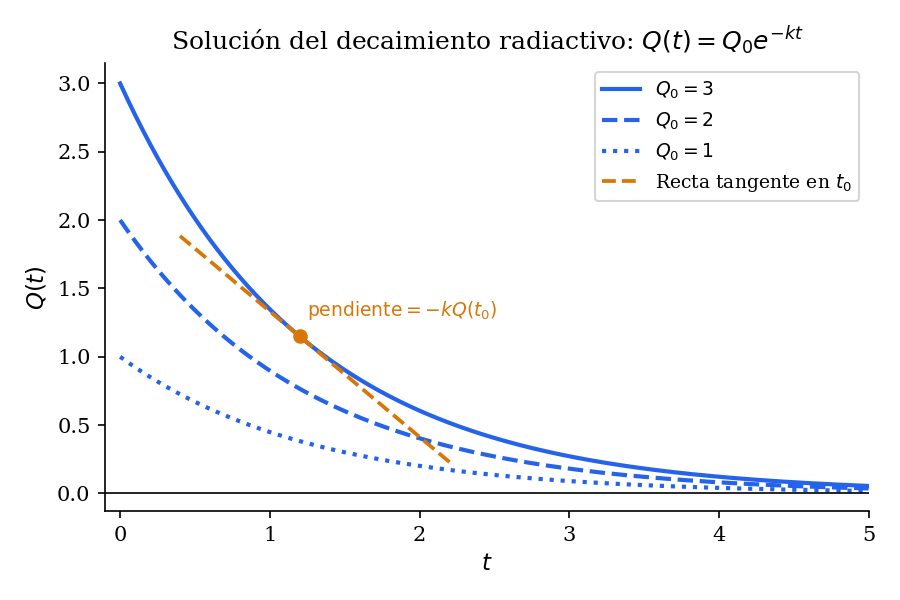
\includegraphics[width=0.72\textwidth]{fig_01_decaimiento_solucion.png}
\caption{Solución $Q(t)=Q_0e^{-kt}$ para distintos valores de $Q_0$.}
\end{figure}

\subsection{Vida media}

\begin{definicion}{Vida media}{}
La \textbf{vida media} $t_{1/2}$ es el tiempo para que la cantidad inicial
se reduzca a la mitad: $Q(t_{1/2})=Q_0/2$.
\end{definicion}

De $Q_0e^{-kt_{1/2}}=Q_0/2$ se obtiene
\[
\boxed{t_{1/2}=\frac{\ln 2}{k}.}
\]
\begin{observacion}{Independencia de $Q_0$}{}
$t_{1/2}$ no depende de la cantidad inicial; es consecuencia de la
estructura exponencial de la solución.
\end{observacion}

\begin{figure}[H]
\centering
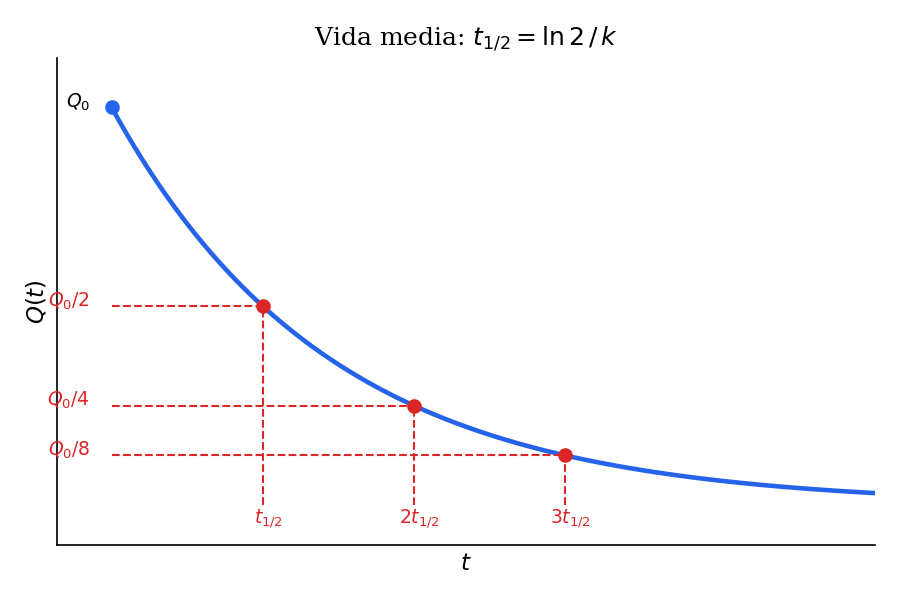
\includegraphics[width=0.72\textwidth]{fig_02_vida_media.png}
\caption{La cantidad se reduce a la mitad en cada intervalo de longitud $t_{1/2}$.}
\end{figure}

% ============================================================
\section{Ecuaciones lineales de primer orden}
\label{sec:ecuaciones-lineales-primer-orden}
% ============================================================

Una ecuación de la forma
\[
\frac{dQ}{dt}+p(t)Q=g(t)
\]
se resuelve mediante el \textbf{factor integrante} $\mu(t)=e^{\int p(t)\dd t}$
(Nagle §2.3). Multiplicando ambos lados por $\mu$:
\[
\frac{d}{dt}\!\bigl[\mu(t)Q(t)\bigr]=\mu(t)g(t),
\]
e integrando se obtiene la solución general.

\subsection{Modelo compartimental con entrada constante}

\textbf{Balance:} entrada $I>0$ menos salida proporcional $kQ$:
\[
\boxed{\frac{dQ}{dt}=-kQ+I,\qquad I>0,\quad k>0.}
\]

\textbf{Punto de equilibrio:} $Q^*=I/k$ (asintóticamente estable).

\textbf{Solución analítica} (factor integrante $e^{kt}$):
\[
\boxed{Q(t)=\frac{I}{k}+\!\left(Q_0-\frac{I}{k}\right)e^{-kt}.}
\]
Para cualquier $Q_0$: $\lim_{t\to\infty}Q(t)=I/k$.

\begin{figure}[H]
\centering
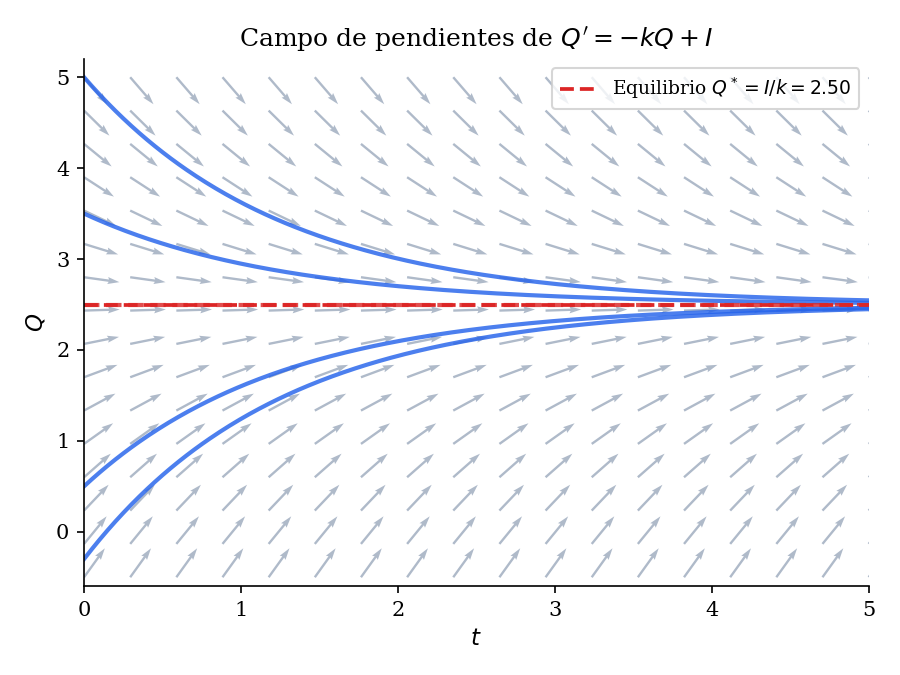
\includegraphics[width=0.74\textwidth]{fig_05_campo_compartimental.png}
\caption{Campo de pendientes de $Q'=-kQ+I$. Todas las trayectorias convergen a
$Q^*=I/k$.}
\end{figure}

\subsection{Circuito RC}
\label{sec:circuito-rc}

Un circuito RC con resistencia $R$, capacitor $C$ y voltaje constante $V_0$
satisface (Nagle §3.5, ley de Kirchhoff):
\[
R\frac{dq}{dt}+\frac{1}{C}q=V_0,
\]
donde $q(t)$ es la carga en el capacitor. Reescribiendo:
\[
\frac{dq}{dt}+\frac{1}{RC}q=\frac{V_0}{R}.
\]
Esta es una ecuación lineal de primer orden con $p=1/(RC)$ y $g=V_0/R$.
Con condición inicial $q(0)=q_0$, la solución es
\[
\boxed{q(t)=CV_0+\bigl(q_0-CV_0\bigr)e^{-t/(RC)}.}
\]
El equilibrio $q^*=CV_0$ es asintóticamente estable con constante de tiempo $\tau_c=RC$.

\textbf{Adimensionalización:} introduciendo
\[
\hat{q}=\frac{q}{CV_0},\qquad \hat{t}=\frac{t}{RC},
\]
la ecuación se reduce a
\[
\frac{d\hat{q}}{d\hat{t}}=1-\hat{q},
\]
que tiene un único parámetro adimensional $\hat{q}^*=1$ y permite estudiar la
dinámica universal del circuito sin depender de $R$, $C$ ni $V_0$.

% ============================================================
\section{Cinética química}
\label{sec:cinetica}
% ============================================================

\subsection{Reacción elemental \texorpdfstring{$A\to B$}{A to B} (primer orden)}

Para la reacción $A\xrightarrow{k}B$ con $A(0)=A_0$, $B(0)=0$:
\[
\boxed{\begin{aligned}
\frac{dA}{dt}&=-kA,\\[4pt]
\frac{dB}{dt}&=kA.
\end{aligned}}
\]

\textbf{Conservación:} sumando las ecuaciones,
$\dfrac{d}{dt}(A+B)=0$, luego
\[
\boxed{A(t)+B(t)=A_0,\qquad t\geq 0.}
\]

\textbf{Solución analítica:}
\[
A(t)=A_0e^{-kt},\qquad
B(t)=A_0\!\left(1-e^{-kt}\right).
\]

\begin{figure}[H]
\centering
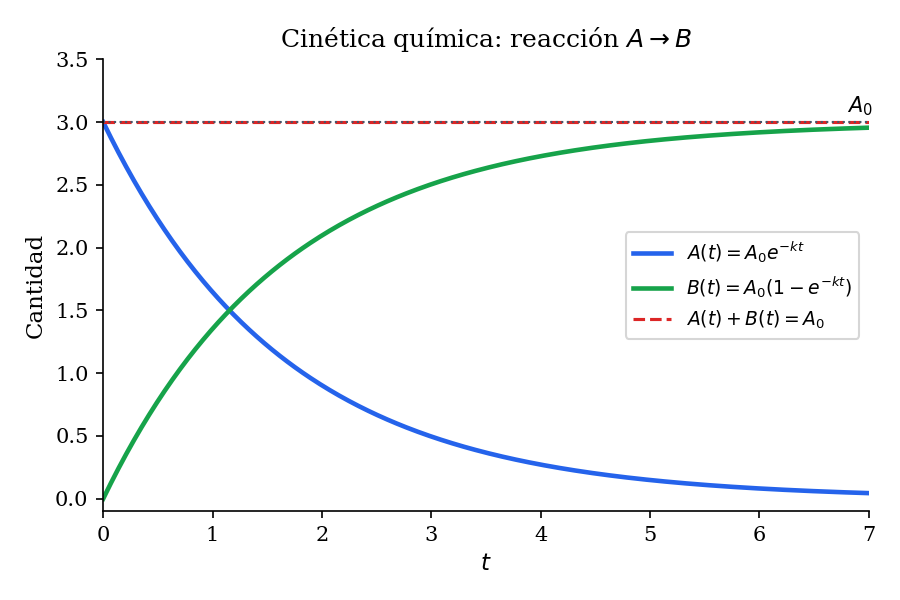
\includegraphics[width=0.72\textwidth]{fig_06_cinetica_AB.png}
\caption{$A(t)$ decrece; $B(t)$ crece. La suma $A+B=A_0$ (línea roja) se conserva.}
\end{figure}

\subsection{Ley de acción de masas}

\begin{definicion}{Ley de acción de masas}{}
Para la reacción $\alpha A+\beta B\xrightarrow{k}\cdots$, la velocidad de
reacción es
\[
v=kA^{\alpha}B^{\beta}.
\]
\end{definicion}

\begin{ejemplo}
\textbf{Reacción $2A\xrightarrow{k}B$.} Por la ley de acción de masas, $v=kA^2$.
Cada reacción consume 2 unidades de $A$ y produce 1 de $B$:
\[
\frac{dA}{dt}=-2kA^2,\qquad \frac{dB}{dt}=kA^2,\qquad A(0)=A_0,\quad B(0)=0.
\]

\textbf{Conservación estequiométrica:}
\[
\frac{d}{dt}(A+2B)=-2kA^2+2kA^2=0
\;\Longrightarrow\;
\boxed{A(t)+2B(t)=A_0.}
\]

\textbf{Solución de $A$:} la ecuación $A'=-2kA^2$ es separable:
\[
\frac{dA}{A^2}=-2k\dd t
\;\Longrightarrow\;
-\frac{1}{A}=-2kt+C.
\]
Con $A(0)=A_0$: $C=-1/A_0$, de modo que
\[
\boxed{A(t)=\frac{A_0}{1+2kA_0 t}.}
\]

\textbf{Solución de $B$:} usando la conservación,
\[
\boxed{B(t)=\frac{A_0}{2}\cdot\frac{2kA_0 t}{1+2kA_0 t}.}
\]

Nótese que $A(t)\to 0$ y $B(t)\to A_0/2$ cuando $t\to\infty$,
verificando $A_0+2\cdot 0=A_0$.
\end{ejemplo}

% ============================================================
\section{Modelos poblacionales}
% ============================================================

\subsection{Modelo malthusiano (Nagle §3.2)}

Bajo hipótesis de crecimiento/mortalidad constantes y sin interacciones:
\[
\boxed{\frac{dN}{dt}=rN,\qquad r\in\mathbb{R}.}
\]
Solución: $N(t)=N_0e^{rt}$.
\begin{itemize}
    \item $r>0$: crecimiento exponencial ($N\to+\infty$).
    \item $r<0$: extinción ($N\to 0$).
    \item $r=0$: población constante.
\end{itemize}

\begin{figure}[H]
\centering
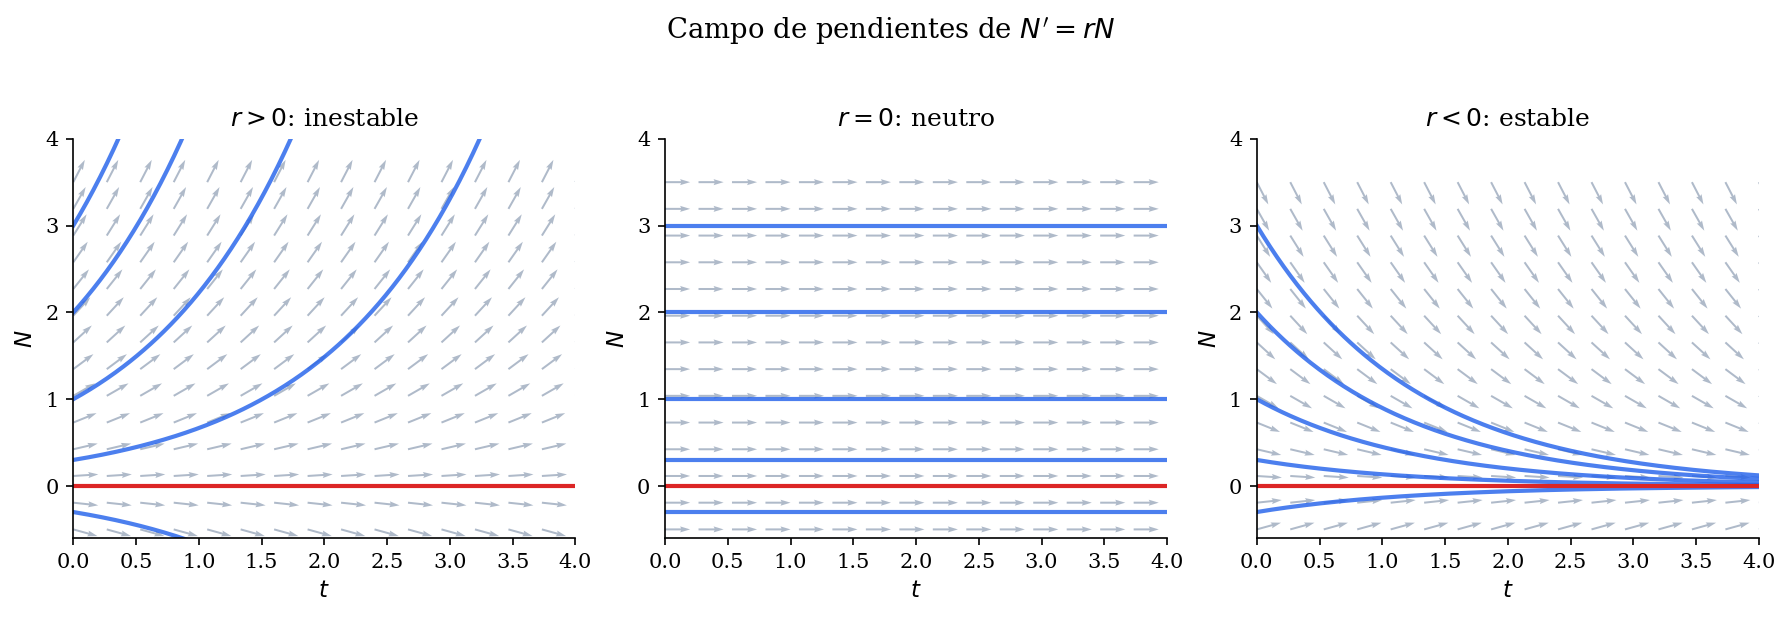
\includegraphics[width=0.92\textwidth]{fig_07_campo_malthusiano.png}
\caption{Campo de pendientes de $N'=rN$ para los tres casos cualitativos.}
\end{figure}

\subsection{Modelo con entrada y salida}

Con generación interna $\gamma$, mortalidad $m$ y entrada exterior $I$:
\[
\frac{dP}{dt}=(\gamma-m)P+I.
\]
El equilibrio es $P^*=I/(m-\gamma)$ (para $m\neq\gamma$) y la solución es
\[
P(t)=P^*+(P_0-P^*)e^{(\gamma-m)t}.
\]

% ============================================================
\section{Ecuaciones diferenciales autónomas}
% ============================================================

\begin{definicion}{Ecuación autónoma}{}
Una ecuación $\dfrac{dy}{dx}=f(y)$ donde el lado derecho \emph{no depende}
explícitamente de $x$ se llama \textbf{autónoma}.
\end{definicion}

\subsection{Puntos de equilibrio}

\begin{definicion}{Punto de equilibrio}{}
$y_0$ es un \textbf{punto de equilibrio} si $f(y_0)=0$.
La función constante $y(x)\equiv y_0$ es solución.
\end{definicion}

\subsection{Línea de fase y análisis geométrico}

El signo de $f(y)$ determina el comportamiento:
\[
f(y)>0\;\Rightarrow\; y'(x)>0\quad(\text{creciente});\qquad
f(y)<0\;\Rightarrow\; y'(x)<0\quad(\text{decreciente}).
\]

\textbf{Procedimiento estándar:}
\begin{enumerate}
    \item Encontrar los equilibrios: $f(y)=0$.
    \item Determinar el signo de $f(y)$ en los intervalos entre equilibrios.
    \item Construir la línea de fase con flechas.
    \item Clasificar cada equilibrio.
    \item Bosquejar cualitativamente las soluciones.
\end{enumerate}

\textbf{Clasificación geométrica:}
\begin{itemize}
    \item \textbf{Estable}: flechas apuntan hacia $y_0$ desde ambos lados.
    \item \textbf{Inestable}: flechas se alejan de $y_0$ por ambos lados.
    \item \textbf{Semiestable}: un lado converge, el otro diverge.
\end{itemize}

\begin{figure}[H]
\centering
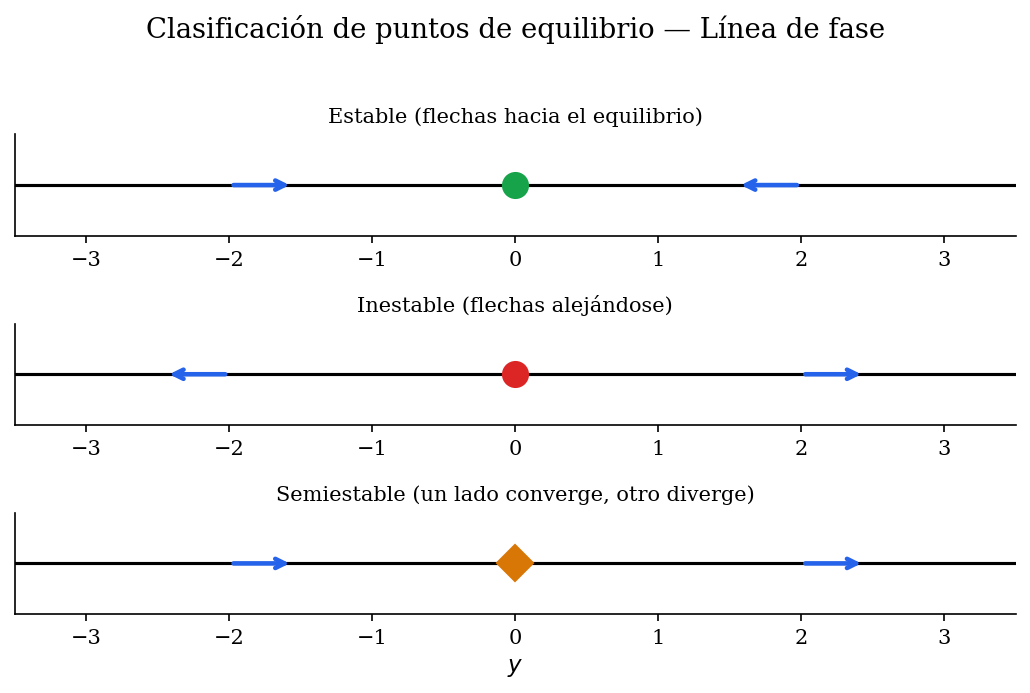
\includegraphics[width=0.74\textwidth]{fig_08_linea_fase_clasificacion.png}
\caption{Clasificación de equilibrios mediante la línea de fase.}
\end{figure}

% ============================================================
\section{Estabilidad y linealización}
% ============================================================

\subsection{Definiciones formales}

\begin{definicion}{Estabilidad de Lyapunov}{}
$y_0$ es \textbf{estable} si para todo $\varepsilon>0$ existe $\delta>0$
tal que $|y(0)-y_0|<\delta\Rightarrow|y(t)-y_0|<\varepsilon$ para todo $t\geq 0$.
\end{definicion}

\begin{definicion}{Estabilidad asintótica}{}
$y_0$ es \textbf{asintóticamente estable} si es estable y además
$|y(0)-y_0|<\delta\Rightarrow\lim_{t\to\infty}y(t)=y_0$.
\end{definicion}

\begin{figure}[H]
\centering
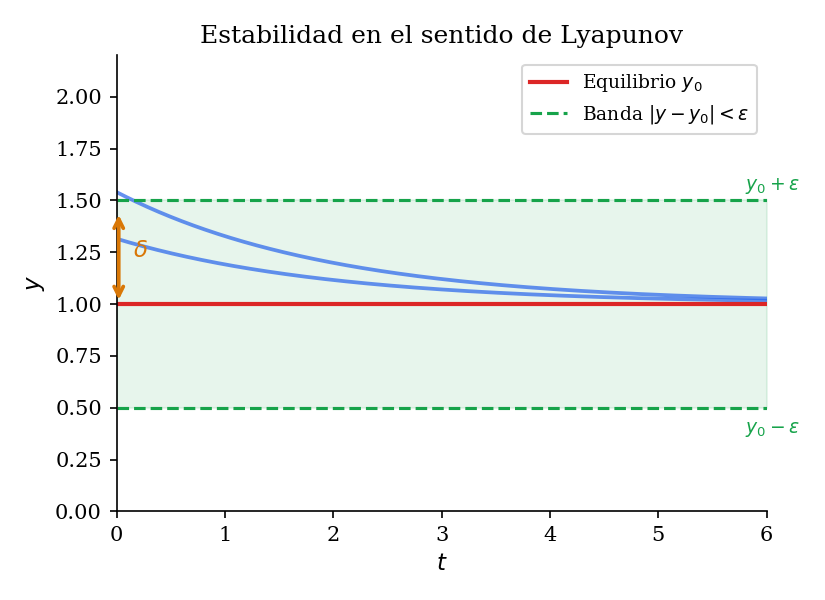
\includegraphics[width=0.62\textwidth]{fig_12_estabilidad_lyapunov.png}
\caption{Estabilidad de Lyapunov: trayectorias dentro de $\delta$ permanecen en $\varepsilon$.}
\end{figure}

\subsection{Criterio de linealización}

Expandiendo $f$ en Taylor alrededor de $y_0$:
\[
f(y)\approx f'(y_0)(y-y_0),\qquad\text{(pues }f(y_0)=0\text{)}.
\]
Con $u(t)=y(t)-y_0$: $u'\approx f'(y_0)u\;\Rightarrow\; u(t)=u(0)e^{f'(y_0)t}$.

\begin{teorema}{Criterio de linealización}{}
Sea $f\in C^1$ y $f(y_0)=0$. Entonces:
\begin{enumerate}[label=\alph*)]
    \item $f'(y_0)<0$: $y_0$ es \textbf{asintóticamente estable}.
    \item $f'(y_0)>0$: $y_0$ es \textbf{inestable}.
    \item $f'(y_0)=0$: el criterio no decide; usar análisis geométrico.
\end{enumerate}
\end{teorema}

\subsection{Linealización en sistemas planos}

Para un sistema autónomo $x'=P(x,y)$, $y'=Q(x,y)$ con equilibrio $X_0=(x_0,y_0)$,
el linealizado es $Y'=J(X_0)Y$ donde
\[
J(x,y)=\begin{pmatrix}
\partial P/\partial x & \partial P/\partial y\\
\partial Q/\partial x & \partial Q/\partial y
\end{pmatrix}.
\]

\begin{teorema}{Hartman--Grobman}{}
Si $J(X_0)$ no tiene autovalores con parte real cero, el retrato de fase
del sistema no lineal cerca de $X_0$ es topológicamente equivalente al
del sistema linealizado $Y'=J(X_0)Y$.
\end{teorema}

% ============================================================
\section{Modelo logístico}
\label{sec:modelo-logistico}
% ============================================================

El modelo logístico introduce la \emph{capacidad de carga} $K>0$:
\[
\boxed{\frac{dN}{dt}=rN\!\left(1-\frac{N}{K}\right),\qquad r,K>0.}
\]

Este es el modelo base de la población con saturación. A partir de él se
obtienen, casi sin cambiar la idea central, las versiones con cosecha y con
efecto Allee que aparecen enseguida.

\subsection{Puntos de equilibrio}

$f(N)=rN(1-N/K)=0\;\Rightarrow\;N_0=0$ y $N_1=K$.

\subsection{Análisis geométrico}

\begin{itemize}
    \item $0<N<K$: $f(N)>0$ $\Rightarrow$ $N$ crece.
    \item $N>K$: $f(N)<0$ $\Rightarrow$ $N$ decrece.
\end{itemize}
Las soluciones con $N_0>0$ tienden a $K$.

\begin{figure}[H]
\centering
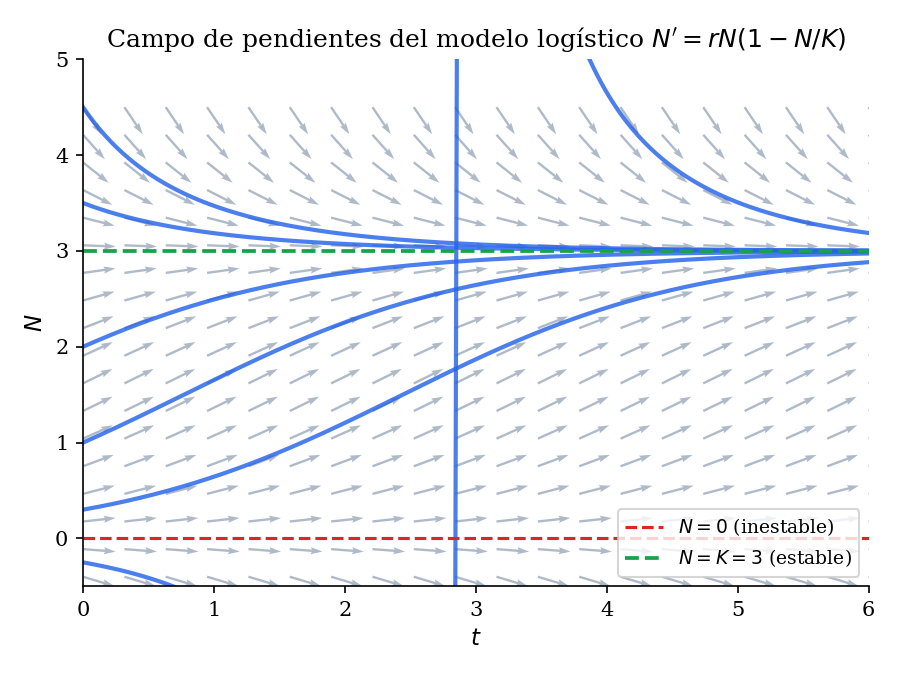
\includegraphics[width=0.72\textwidth]{fig_09_campo_logistico.png}
\caption{Campo de pendientes del logístico. Soluciones sigmoidales convergen a $K$.}
\end{figure}

\begin{figure}[H]
\centering
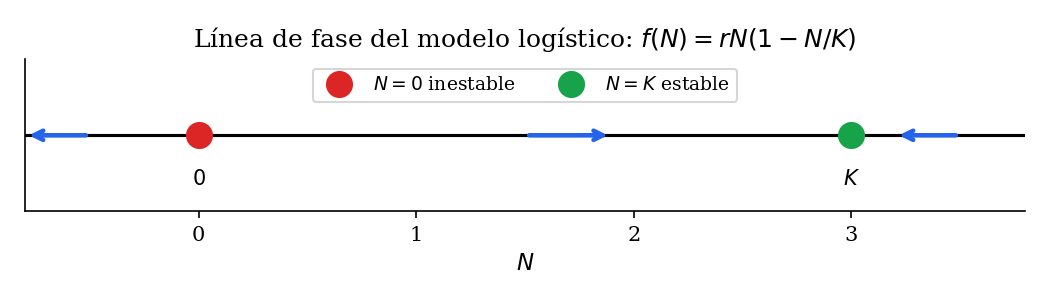
\includegraphics[width=0.70\textwidth]{fig_10_linea_fase_logistico.png}
\caption{Línea de fase: $N=0$ inestable, $N=K$ asintóticamente estable.}
\end{figure}

\subsection{Linealización}

$f'(N)=r-2rN/K$.
\[
f'(0)=r>0\;\Rightarrow\; N=0\text{ inestable}.\qquad
f'(K)=-r<0\;\Rightarrow\; N=K\text{ a.e.}
\]

\subsection{Solución analítica}

La ecuación es separable. Con fracciones parciales:
\[
\frac{K}{N(K-N)}=\frac{1}{N}+\frac{1}{K-N},
\]
integrando y usando $N(0)=N_0$ se obtiene
\[
\boxed{N(t)=\frac{K}{1+\displaystyle\left(\frac{K-N_0}{N_0}\right)e^{-rt}}.}
\]

Una vez resuelto el caso base, conviene mirar dos extensiones muy comunes:
la extracción constante y el efecto Allee. Ambas conservan la misma lógica de
equilibrios, pero cambian de forma importante la estabilidad.

\subsection{Modelo logístico con cosecha}

Con extracción constante $H>0$:
\[
\frac{dN}{dt}=rN\!\left(1-\frac{N}{K}\right)-H.
\]
Los equilibrios satisfacen $N^*=\dfrac{K}{2}\!\left(1\pm\sqrt{1-4H/(rK)}\right)$.
Existen tres regímenes según $H$ comparado con $rK/4$.

\begin{figure}[H]
\centering
\begin{tikzpicture}
\begin{axis}[
    width=0.94\textwidth, height=5.2cm,
    xmin=0, xmax=0.40, ymin=-0.05, ymax=1.05,
    axis lines=middle,
    xlabel={$\lambda=H/(rK)$}, ylabel={$u^*=N/K$},
    title={Bifurcaci\'on silla-nodo del log\'istico con cosecha},
    samples=200, tick style={draw=none}
]
\addplot[thick,blue!75!black,domain=0:0.249] ({x},{0.5 - sqrt(0.25 - x)});
\addplot[thick,blue!75!black,domain=0:0.249] ({x},{0.5 + sqrt(0.25 - x)});
\addplot[thick,red!70!black,dashed] coordinates {(0.25,0) (0.25,1)};
\node[anchor=west] at (axis cs:0.258,0.95) {$\lambda=\frac14$};
\end{axis}
\end{tikzpicture}
\caption{Bifurcación silla-nodo: los dos equilibrios colisionan en $\lambda=1/4$.}
\end{figure}

\subsection{Modelo logístico con efecto Allee}

Si el crecimiento cambia de signo para poblaciones bajas:
\[
\frac{dN}{dt}=rN\!\left(1-\frac{N}{K}\right)\!\left(\frac{N}{A}-1\right),
\qquad r>0,\; 0<A<K.
\]
Equilibrios: $N_0=0$ (estable), $N_1=A$ (inestable), $N_2=K$ (estable).

\begin{figure}[H]
\centering
\begin{tikzpicture}
\begin{axis}[
    width=0.92\textwidth, height=6cm,
    xmin=0, xmax=2, ymin=-0.05, ymax=1.15,
    axis lines=middle,
    xlabel={$\lambda=A/K$}, ylabel={$u^*=N/K$},
    tick style={draw=none},
    title={Bifuraci\'on transcr\'itica del efecto Allee},
    samples=200
]
\addplot[thick,blue!70!black,domain=0:2] {0};
\addplot[thick,blue!70!black,domain=0:1] {1};
\addplot[thick,blue!70!black,dashed,domain=1:2] {1};
\addplot[thick,blue!70!black,dashed,domain=0:1] {x};
\addplot[thick,blue!70!black,domain=1:2] {x};
\addplot[only marks,mark=*,mark size=1.5pt] coordinates {(1,1)};
\end{axis}
\end{tikzpicture}
\caption{Las ramas no triviales intercambian estabilidad en $\lambda=A/K=1$.}
\end{figure}

% ============================================================
\section{Bifurcaciones en sistemas unidimensionales}
\label{sec:bifurcaciones-unidim}
% ============================================================

Los dos ejemplos anteriores muestran que, al variar un parámetro, los puntos de
equilibrio pueden aparecer, desaparecer o intercambiar estabilidad. Esa es la
idea de bifurcación en una dimensión, y aquí la ordenamos en los tipos más
estándar.

\begin{definicion}{Bifurcación}{}
Se dice que $\mu_0$ es un \textbf{valor de bifurcación} de $y'=f(y,\mu)$
si al cruzar $\mu_0$ cambia el número o la estabilidad de los equilibrios.
\end{definicion}

El \textbf{diagrama de bifurcación} grafica los equilibrios $y^*(\mu)$ en el
plano $(\mu,y^*)$, usando línea sólida para ramas estables y línea discontinua
para inestables.

\subsection{Bifurcación silla-nodo}

Dos equilibrios (uno estable, uno inestable) se crean o destruyen al variar $\mu$.

\textbf{Ejemplo canónico:} $y'=y^2+\mu$.
\begin{itemize}
    \item $\mu<0$: equilibrios $y^*=\pm\sqrt{-\mu}$; $y^*=-\sqrt{-\mu}$ estable, $y^*=\sqrt{-\mu}$ inestable.
    \item $\mu=0$: único equilibrio $y^*=0$ semiestable (bifurcación).
    \item $\mu>0$: no hay equilibrios.
\end{itemize}
Verificación por linealización: $f'(y)=2y$, de modo que
$f'(-\sqrt{-\mu})=-2\sqrt{-\mu}<0$ (estable) y $f'(\sqrt{-\mu})=2\sqrt{-\mu}>0$ (inestable).

\textbf{Variante:} $y'=\mu+y-y^3$.
Los equilibrios satisfacen $\mu=y^3-y$. Al graficar $\mu$ frente a $y$
se observa que para ciertos rangos de $\mu$ coexisten tres soluciones;
hay dos valores de bifurcación silla-nodo donde la curva $\mu=y^3-y$
tiene extremos locales.

\subsection{Bifurcación transcrítica}

Dos equilibrios existen para todo $\mu$ pero \emph{intercambian estabilidad}
al cruzar $\mu_0$.

\textbf{Ejemplo canónico:} $y'=\mu y-y^2=y(\mu-y)$.
\begin{itemize}
    \item Equilibrios: $y^*=0$ y $y^*=\mu$ para todo $\mu$.
    \item $f'(y)=\mu-2y$.
    \item $\mu<0$: $f'(0)=\mu<0$ ($y=0$ estable); $f'(\mu)=-\mu>0$ ($y=\mu$ inestable).
    \item $\mu>0$: $f'(0)=\mu>0$ ($y=0$ inestable); $f'(\mu)=-\mu<0$ ($y=\mu$ estable).
    \item $\mu=0$: ambos equilibrios coinciden; linealización no decide.
\end{itemize}

\textbf{Variante:} $y'=y(\mu-y)$. Idéntico análisis; el equilibrio $y=\mu$
tiene interpretación como nivel de saturación ambiental en modelos poblacionales.

\subsection{Bifurcación pitchfork supercrítica}

Un equilibrio estable se divide en tres al cruzar $\mu_0$: el central se
vuelve inestable y nacen dos nuevos estables.

\textbf{Ejemplo canónico:} $y'=\mu y-y^3$.
\begin{itemize}
    \item Equilibrios: $y^*=0$ y (para $\mu>0$) $y^*=\pm\sqrt{\mu}$.
    \item $f'(y)=\mu-3y^2$.
    \item $\mu\leq 0$: $f'(0)=\mu\leq 0$; solo $y=0$, estable.
    \item $\mu>0$: $f'(0)=\mu>0$ ($y=0$ inestable); $f'(\pm\sqrt{\mu})=-2\mu<0$ (estables).
\end{itemize}
Nombre ``supercrítica'': las ramas nuevas aparecen \emph{del lado} $\mu>0$.

\textbf{Variante equivalente:} $y'=y(\mu-y^2)$. Mismo análisis factorizando.

\subsection{Bifurcación pitchfork subcrítica}

\textbf{Ejemplo canónico:} $y'=\mu y+y^3$.
\begin{itemize}
    \item Equilibrios: $y^*=0$ y (para $\mu<0$) $y^*=\pm\sqrt{-\mu}$.
    \item $f'(y)=\mu+3y^2$.
    \item $\mu<0$: $f'(0)=\mu<0$ ($y=0$ estable); $f'(\pm\sqrt{-\mu})=-2\mu>0$
          ($y^*=\pm\sqrt{-\mu}$ \emph{inestables}).
    \item $\mu>0$: $f'(0)=\mu>0$ ($y=0$ inestable); no hay equilibrios adicionales.
\end{itemize}
Nombre ``subcrítica'': las ramas inestables existen para $\mu<0$
(antes del punto de bifurcación). El sistema presenta \emph{histéresis}.

\subsection{Resumen de tipos}

\begin{center}
\begin{tabular}{lll}
\toprule
Tipo & Ejemplo & Característica\\
\midrule
Silla-nodo & $y'=y^2+\mu$ & se crean/destruyen 2 equilibrios\\
Transcrítica & $y'=\mu y-y^2$ & intercambio de estabilidad\\
Pitchfork supercrítica & $y'=\mu y-y^3$ & bifurcación con simetría $y\leftrightarrow -y$\\
Pitchfork subcrítica & $y'=\mu y+y^3$ & ramas inestables; histéresis\\
Bifurcación periódica & $\dot\theta=\mu\sin\theta$ & infinitos equilibrios periódicos\\
Cúspide (codim.~2) & $y'=y^3-3\mu y+\mu$ & requiere dos parámetros\\
\bottomrule
\end{tabular}
\end{center}

% ============================================================
\subsection{Bifurcación periódica: flujos en el círculo}
% ============================================================

Los ejercicios anteriores viven en la \emph{recta}. Cuando la variable de estado
es un \emph{ángulo} $\theta\in[0,2\pi)$, el espacio de fases es el \textbf{círculo},
y aparecen fenómenos nuevos: las soluciones pueden ser \emph{periódicas} aunque el
sistema sea unidimensional (Strogatz, Cap.~4).

\begin{definicion}{Campo vectorial en el círculo}{}
Una ecuación $\dot\theta=f(\theta)$ donde $f$ es $2\pi$-periódica,
$f(\theta+2\pi)=f(\theta)$, define un \textbf{campo vectorial en el círculo}.
Los puntos de equilibrio son $\theta^*$ tales que $f(\theta^*)=0$.
A diferencia de la recta, una partícula que fluye en una dirección puede
\emph{regresar} a su punto de partida, generando soluciones periódicas.
\end{definicion}

\textbf{Ejemplo canónico de la tarea:} $\dot\theta=\mu\sin\theta$, con
$\mu\in\mathbb{R}$ parámetro de control.

\textbf{Análisis:}
\begin{itemize}
  \item Los equilibrios satisfacen $\sin\theta^*=0$, es decir
        $\theta^*=0$ y $\theta^*=\pi$ (y sus traslados $2\pi k$), para \emph{todo} $\mu\neq 0$.
  \item $f'(\theta)=\mu\cos\theta$. Entonces:
        \begin{itemize}
            \item En $\theta^*=0$: $f'(0)=\mu$.
                  Si $\mu>0$ es \textbf{inestable}; si $\mu<0$ es \textbf{estable}.
            \item En $\theta^*=\pi$: $f'(\pi)=-\mu$.
                  Si $\mu>0$ es \textbf{estable}; si $\mu<0$ es \textbf{inestable}.
        \end{itemize}
  \item En $\mu=0$: $\dot\theta=0$, todos los puntos son equilibrios
        (caso degenerado, la linealización no decide).
\end{itemize}

\textbf{Diagrama de bifurcación:} al cruzar $\mu=0$ los dos equilibrios
$\theta^*=0$ y $\theta^*=\pi$ \emph{intercambian estabilidad}
(bifurcación de tipo transcrítico en el círculo).
Para $\mu\neq 0$ existen exactamente dos equilibrios en $[0,2\pi)$, uno
estable y uno inestable.

\begin{observacion}{Multiplicidad periódica}{}
Como $f(\theta)=\mu\sin\theta$ es $2\pi$-periódica, en el círculo
hay infinitos equilibrios: $\theta^*=k\pi$, $k\in\mathbb{Z}$.
El diagrama de bifurcación se repite periódicamente y todos ellos
intercambian estabilidad simultáneamente al cruzar $\mu=0$.
\end{observacion}

% ============================================================
\subsection{Bifurcación de cúspide (codimensión 2)}
% ============================================================

Todos los tipos anteriores son \emph{codimensión~1}: basta variar un solo
parámetro para que ocurra la bifurcación. La \textbf{cúspide} es de
\emph{codimensión~2}: necesitamos ajustar \emph{dos} parámetros simultáneamente
para alcanzar el punto de bifurcación (Strogatz, §3.6).

\textbf{Ejemplo canónico de la tarea:} $y'=y^3-3\mu y+\mu$ (o la forma
estándar $\dot x = h + rx - x^3$, que tiene la misma estructura).

Trabajamos con la \textbf{forma normal de la cúspide}:
\[
\dot{x} = h + rx - x^3,
\]
que tiene dos parámetros de control: $r$ (bifurcación) y $h$ (imperfección).

\textbf{Puntos de equilibrio:} satisfacen $x^3-rx=h$. Estudiamos la función
$g(x)=x^3-rx$ y buscamos intersecciones con la horizontal $y=h$.

\textbf{Número de equilibrios según $(r,h)$:}
\begin{itemize}
    \item Si $r\leq 0$: $g(x)$ es monótona creciente $\Rightarrow$ exactamente
          \textbf{1 equilibrio} para todo $h$.
    \item Si $r>0$: $g(x)$ tiene un máximo local en $x_{\max}=-\sqrt{r/3}$
          con valor $g(x_{\max})=\frac{2}{3}(r/3)^{3/2}$ y un mínimo en
          $x_{\min}=\sqrt{r/3}$ con valor $-\frac{2}{3}(r/3)^{3/2}$.
          Define $h_c(r)=\frac{2}{3}(r/3)^{3/2}$.
          \begin{itemize}
              \item $|h|<h_c(r)$: \textbf{3 equilibrios} (2 estables, 1 inestable).
              \item $|h|=h_c(r)$: \textbf{2 equilibrios} (bifurcación silla-nodo).
              \item $|h|>h_c(r)$: \textbf{1 equilibrio}.
          \end{itemize}
\end{itemize}

\textbf{Conjunto de bifurcación} (curvas en el plano $(r,h)$ donde ocurren
sillas-nodo):
\[
h = \pm h_c(r) = \pm\frac{2}{3}\left(\frac{r}{3}\right)^{3/2},\qquad r>0.
\]
Las dos curvas se unen tangencialmente en el \textbf{punto de cúspide}
$(r,h)=(0,0)$, que es la bifurcación de codimensión~2.

\begin{observacion}{Histéresis y catástrofe}{}
Al variar $h$ con $r>0$ fijo, si el sistema está en el equilibrio superior
estable y $h$ supera $h_c(r)$, ese equilibrio desaparece y el sistema
\emph{salta discontinuamente} al equilibrio inferior.
Al regresar $h$, el salto de vuelta ocurre en $h=-h_c(r)$.
Este comportamiento irreversible se llama \textbf{catástrofe de cúspide}
y genera \textbf{histéresis}: la trayectoria de ida y la de vuelta son diferentes.
\end{observacion}

\textbf{Aplicación al ejercicio (j):} $y'=y^3-3\mu y+\mu$.
Comparando con $\dot x=h+rx-x^3$, identificamos $r=3\mu$ y $h=\mu$.
La curva paramétrica de bifurcación es:
\[
\mu=h=h_c(r)=h_c(3\mu)=\frac{2}{3}\left(\mu\right)^{3/2},
\]
lo que da la condición $\mu=0$ (punto de cúspide) y las curvas de silla-nodo
para $\mu>0$. Para $\mu$ pequeño, el sistema tiene un único equilibrio;
para valores mayores, tres. El diagrama de bifurcación en $\mu$ muestra
la aparición y colapso de ramas en un punto de tipo cúspide.

% ============================================================
\section{Ejemplo de ecuación cuadrática: \texorpdfstring{$y'=y^2+\alpha$}{y prime = y squared + alpha}}
% ============================================================

Consideremos
\[
\frac{dy}{dx}=y^2+\alpha,\qquad\alpha\in\mathbb{R}.
\]

\textbf{Caso $\alpha<0$:} equilibrios $y_1=-\sqrt{-\alpha}$ (estable) y
$y_2=\sqrt{-\alpha}$ (inestable). Verificación: $f'(y)=2y$.

\textbf{Caso $\alpha=0$:} único equilibrio $y=0$ semiestable ($f'(0)=0$;
linealización no decide, se usa análisis geométrico).

\textbf{Caso $\alpha>0$:} no hay equilibrios; todas las soluciones crecen.

El valor $\alpha=0$ es un valor de bifurcación silla-nodo.

\begin{figure}[H]
\centering
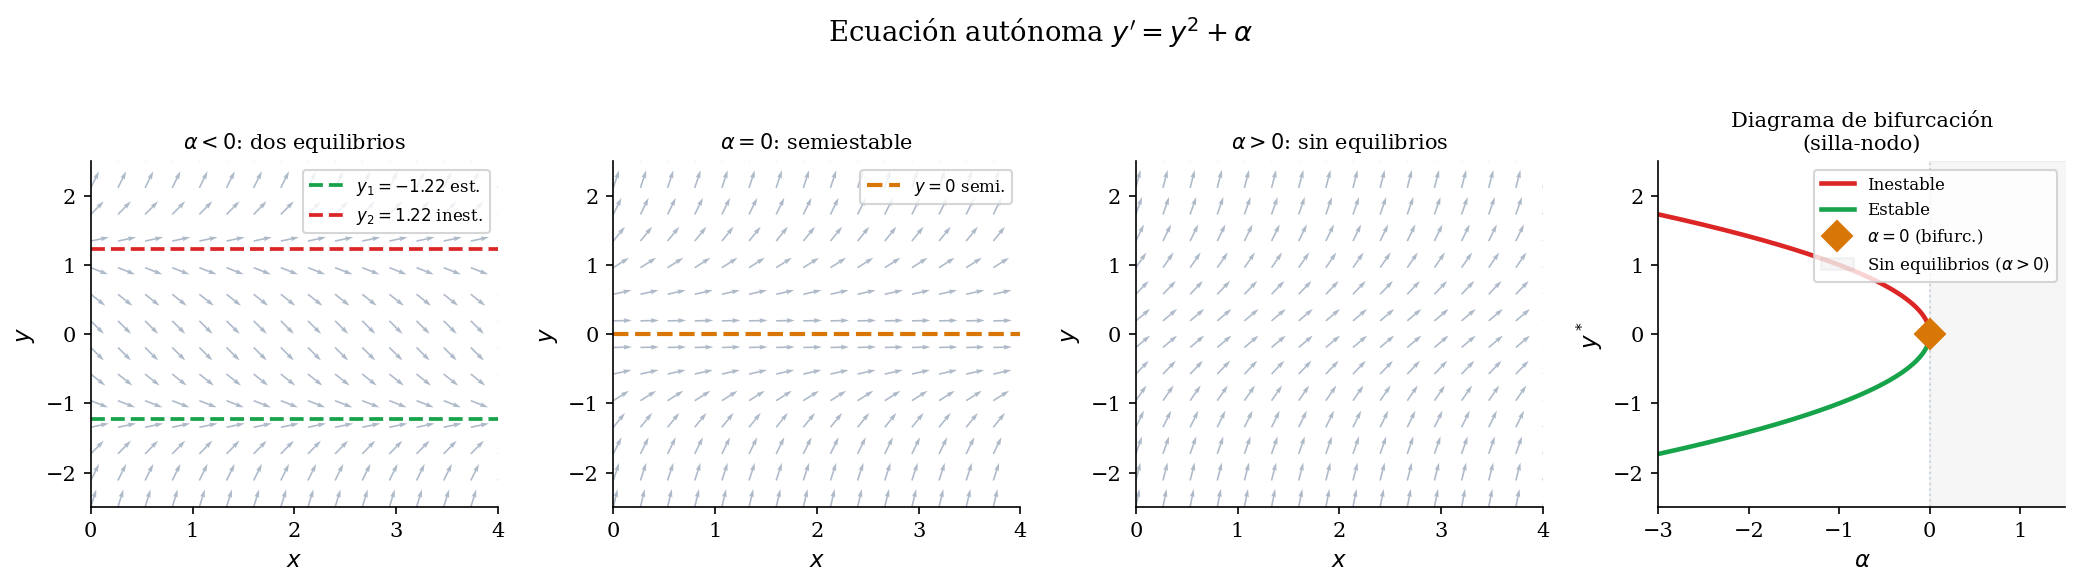
\includegraphics[width=\textwidth]{fig_11_autonoma_bifurcacion.png}
\caption{Campos de pendientes y diagrama de bifurcación de $y'=y^2+\alpha$.}
\end{figure}

% ============================================================
\section{Dinámica de dos poblaciones: Lotka--Volterra}
\label{sec:lotka-volterra}
% ============================================================

Después de estudiar una sola población, pasamos al caso de dos especies
interactuando. El sistema clásico presa--depredador es (Nagle §5.1):
\[
\frac{dx}{dt}=ax-bxy,\qquad
\frac{dy}{dt}=-cy+dxy,\qquad a,b,c,d>0,
\]
donde $x(t)$ es la presa e $y(t)$ el depredador.

\subsection{Equilibrios}

$(0,0)$ y $(x^*,y^*)=(c/d,\, a/b)$.

\subsection{Adimensionalización}

Se introducen variables características:
\[
x=u\,x_c,\quad y=v\,y_c,\quad t=\tau\,t_c.
\]
Para eliminar todos los parámetros libres se elige
\[
x_c=\frac{c}{d},\qquad y_c=\frac{a}{b},\qquad t_c=\frac{1}{a}.
\]

Sustituyendo, la ecuación de $x$ se convierte en:
\[
\frac{x_c}{t_c}\frac{du}{d\tau}=a(x_c u)-b(x_c u)(y_c v)
\;\Longrightarrow\;
\frac{du}{d\tau}=u(1-v).
\]
Análogamente, la ecuación de $y$ queda:
\[
\frac{dy_c}{t_c}\frac{dv}{d\tau}=-c(y_c v)+d(x_c u)(y_c v)
\;\Longrightarrow\;
\frac{dv}{d\tau}=-\frac{c}{a}v+\frac{d\,x_c}{a}uv.
\]
Con $x_c=c/d$: $d\,x_c/a=c/a$, de modo que
\[
\boxed{\frac{du}{d\tau}=u(1-v),\qquad
\frac{dv}{d\tau}=\delta v(u-1),\qquad \delta=\frac{c}{a}.}
\]
El sistema adimensional tiene un \emph{solo} parámetro $\delta=c/a$ en lugar de cuatro.
Los equilibrios son $(0,0)$ y $(1,1)$.
Este reescalamiento deja la estructura dinámica esencial a la vista y facilita
compararlo con las variantes más generales que aparecen después.

\begin{figure}[H]
\centering
\begin{minipage}[t]{0.56\textwidth}
\centering
\begin{tikzpicture}[scale=0.95]
\draw[->] (0,0) -- (7,0) node[right] {$P$};
\draw[->] (0,0) -- (0,5.5) node[above] {$D$};
\draw[thick,blue!70!black] (0,4.6) -- (4.6,0)
    node[pos=0.85,above] {$D=\frac{r}{\beta}\!\left(1-\frac{P}{K}\right)$};
\draw[thick,red!70!black,dashed] (3.0,0) -- (3.0,5.2) node[above] {$P=\frac{\gamma}{\delta}$};
\fill (3.0,1.55) circle (2pt) node[above right] {$E^*$};
\foreach \x/\y in {0.8/0.8,1.5/1.2,2.0/2.7,3.8/1.0,4.8/2.8,2.0/4.0,4.8/4.2}{
  \pgfmathsetmacro{\u}{(\x*(1-\x/4)-0.45*\x*\y)}
  \pgfmathsetmacro{\v}{(-\y+0.35*\x*\y)}
  \pgfmathsetmacro{\len}{sqrt(\u*\u+\v*\v)}
  \draw[-{Latex[length=2mm]},gray!70] (\x,\y)--++({0.48*\u/\len},{0.48*\v/\len});
}
\end{tikzpicture}
\end{minipage}
\hfill
\begin{minipage}[t]{0.40\textwidth}
\centering
\begin{tikzpicture}
\begin{axis}[
    width=\linewidth, height=4.8cm,
    xmin=0,xmax=5,ymin=0,ymax=5,
    axis lines=middle,
    xlabel={$P$},ylabel={$f(P)$},
    tick style={draw=none},xtick=\empty,ytick=\empty,
    legend style={draw=none,at={(0.02,0.98)},anchor=north west,font=\small}
]
\addplot[thick,red!70!black,domain=0:5,samples=200]{x};
\addlegendentry{$f=P$}
\addplot[thick,blue!70!black,domain=0:5,samples=200]{x/(1+x)};
\addlegendentry{$f=\frac{P}{1+P}$}
\end{axis}
\end{tikzpicture}
\end{minipage}
\caption{Plano de fases presa-depredador y respuestas funcionales típicas.}
\end{figure}

% ============================================================
\section{Adimensionalización}
\label{sec:adimensionalizacion}
% ============================================================

La \textbf{adimensionalización} (o normalización) es el proceso de eliminar
unidades físicas de una ecuación diferencial mediante cambios de variable
apropiados, reduciendo el número de parámetros relevantes.

Aquí se resume la técnica general que ya se fue usando en los ejemplos
anteriores: elegir escalas características, redefinir variables y conservar
solo los parámetros que realmente gobiernan la dinámica.

\begin{definicion}{Análisis dimensional}{}
Si $[Q]$ denota la dimensión de la cantidad $Q$, una ecuación diferencial
está \textbf{adimensionalizada} si y solo si todas las variables y parámetros
que aparecen en ella son adimensionales, es decir, tienen dimensión $1$ (sin unidades).
\end{definicion}

\textbf{Procedimiento general:}
\begin{enumerate}
    \item Identificar las variables y parámetros \emph{con} dimensiones.
    \item Construir \emph{escalas características} $[x_c]$, $[t_c]$, etc.,
          a partir de los parámetros del problema.
    \item Definir variables adimensionales, p.~ej.\ $\hat{x}=x/x_c$,
          $\hat{t}=t/t_c$.
    \item Sustituir en la ecuación y verificar que el resultado no tiene unidades.
    \item Identificar los parámetros adimensionales que controlan la dinámica.
\end{enumerate}

\subsection{Análisis dimensional del modelo logístico}

Para $dN/dt=rN(1-N/K)$, las dimensiones son:
\[
[N]=[K]=\text{individuos}\equiv\mathcal{N},\qquad
[r]=T^{-1},\qquad
[t]=T.
\]
Cada término tiene dimensión $\mathcal{N}T^{-1}$, lo que es consistente.

\textbf{Cambio de variables:} $u=N/K$ (adimensional), $\tau=rt$ (adimensional):
\[
\frac{du}{d\tau}=u(1-u).
\]
Esta ecuación no tiene parámetros: todos fueron absorbidos por las escalas.

\subsection{Adimensionalización del logístico con cosecha}

Para $dN/dt=rN(1-N/K)-H$, el análisis dimensional da $[H]=\mathcal{N}T^{-1}$.
Con $u=N/K$ y $\tau=rt$:
\[
\frac{du}{d\tau}=u(1-u)-\lambda,\qquad \lambda=\frac{H}{rK}.
\]

\textbf{Verificación:} $[\lambda]=[H]/([r][K])=(\mathcal{N}T^{-1})/(T^{-1}\cdot\mathcal{N})=1$.
La ecuación está correctamente adimensionalizada.

\subsection{Adimensionalización del efecto Allee}

Para
\[
\frac{dN}{dt}=rN\!\left(1-\frac{N}{K}\right)\!\left(\frac{N}{A}-1\right),
\]
con $u=N/K$ y $\tau=rt$, cada factor:
\begin{itemize}
    \item $N/K=u$: adimensional \checkmark
    \item $N/A=(K/A)u=u/\lambda$, con $\lambda=A/K$: adimensional \checkmark
\end{itemize}
El resultado es:
\[
\frac{du}{d\tau}=u(1-u)\!\left(\frac{u}{\lambda}-1\right),
\qquad \lambda=\frac{A}{K}.
\]

\textbf{Verificación dimensional:} $[\lambda]=[A]/[K]=\mathcal{N}/\mathcal{N}=1$ \checkmark.
La ecuación adimensionalizada tiene un único parámetro $\lambda=A/K$.

\subsection{Caída libre con resistencia lineal (Nagle §3.4)}

Una partícula de masa $m$ cae bajo gravedad $g$ con resistencia proporcional
a la velocidad:
\[
m\frac{dv}{dt}=mg-kv,\qquad k>0.
\]

\textbf{Dimensiones:} $[v]=LT^{-1}$, $[g]=LT^{-2}$, $[k]=MT^{-1}$,
$[m]=M$.

\textbf{Velocidad característica} (velocidad terminal, equilibrio del sistema):
imponiendo $dv/dt=0$:
\[
v_\infty=\frac{mg}{k}.
\]
\textbf{Tiempo característico:} $t_c=m/k$ (tiempo de relajación).

\textbf{Variable adimensional:} $\hat{v}=v/v_\infty=kv/(mg)$,\quad
$\hat{t}=t/t_c=kt/m$.

Sustituyendo:
\[
\frac{v_\infty}{t_c}\frac{d\hat{v}}{d\hat{t}}=g-\frac{k}{m}v_\infty\hat{v}
=g-g\hat{v}=g(1-\hat{v}).
\]
Como $v_\infty/t_c=(mg/k)/(m/k)=g$:
\[
\boxed{\frac{d\hat{v}}{d\hat{t}}=1-\hat{v}.}
\]
La ecuación adimensional no tiene parámetros. El único equilibrio $\hat{v}=1$
(que corresponde a $v=v_\infty=mg/k$) es asintóticamente estable.

\textbf{Solución:} con $\hat{v}(0)=\hat{v}_0$:
$\hat{v}(\hat{t})=1-(1-\hat{v}_0)e^{-\hat{t}}$, es decir,
\[
v(t)=v_\infty\!\left[1-\!\left(1-\frac{v_0}{v_\infty}\right)e^{-kt/m}\right].
\]

\subsection{Oscilador armónico amortiguado (Nagle §4.1, §4.9)}

La ecuación de movimiento de una masa $m$ sujeta a un resorte de rigidez $k$
con amortiguamiento $c\geq 0$ es:
\[
m\frac{d^2x}{dt^2}+c\frac{dx}{dt}+kx=0,\qquad m,k>0,\;c\geq 0.
\]

\textbf{Dimensiones:} $[x]=L$, $[m]=M$, $[k]=MT^{-2}$, $[c]=MT^{-1}$.

\textbf{Escalas características:}
\begin{itemize}
    \item \emph{Tiempo:} frecuencia natural $\omega_0=\sqrt{k/m}$, con $[\omega_0]=T^{-1}$,
          de modo que $t_c=1/\omega_0=\sqrt{m/k}$.
    \item \emph{Longitud:} cualquier longitud de referencia $x_c$ (p.~ej.\ la amplitud inicial $x_0$).
\end{itemize}

\textbf{Variables adimensionales:} $\hat{x}=x/x_c$,\quad $\tau=\omega_0 t=t\sqrt{k/m}$.

Calculando las derivadas:
\[
\frac{dx}{dt}=x_c\omega_0\frac{d\hat{x}}{d\tau},\qquad
\frac{d^2x}{dt^2}=x_c\omega_0^2\frac{d^2\hat{x}}{d\tau^2}.
\]
Sustituyendo y dividiendo entre $mx_c\omega_0^2=kx_c$:
\[
\boxed{\frac{d^2\hat{x}}{d\tau^2}+2\zeta\frac{d\hat{x}}{d\tau}+\hat{x}=0,}
\]
donde el único parámetro adimensional es el \textbf{factor de amortiguamiento}:
\[
\zeta=\frac{c}{2\sqrt{mk}}.
\]

Clasificación por $\zeta$:
\begin{itemize}
    \item $\zeta<1$: subamortiguado (oscilaciones decrecientes).
    \item $\zeta=1$: críticamente amortiguado.
    \item $\zeta>1$: sobreamortiguado (sin oscilaciones).
\end{itemize}

\subsection{Péndulo simple (Nagle §4.8)}

El ángulo $\theta(t)$ de un péndulo de longitud $L$ satisface:
\[
\frac{d^2\theta}{dt^2}+\frac{g}{L}\sin\theta=0.
\]

\textbf{Escala temporal natural:} $\omega_0=\sqrt{g/L}$, de modo que $t_c=\sqrt{L/g}$.

\textbf{Variable adimensional:} $\tau=t/t_c=t\sqrt{g/L}$.

Calculando:
\[
\frac{d\theta}{dt}=\frac{1}{t_c}\frac{d\theta}{d\tau},\qquad
\frac{d^2\theta}{dt^2}=\frac{1}{t_c^2}\frac{d^2\theta}{d\tau^2}=\frac{g}{L}\frac{d^2\theta}{d\tau^2}.
\]
Sustituyendo:
\[
\frac{g}{L}\frac{d^2\theta}{d\tau^2}+\frac{g}{L}\sin\theta=0.
\]
Dividiendo entre $g/L$:
\[
\boxed{\frac{d^2\theta}{d\tau^2}+\sin\theta=0.}
\]
La ecuación adimensionalizada no tiene parámetros. La escala
$t_c=\sqrt{L/g}$ es la \emph{única} combinación de $L$ y $g$ con dimensión de tiempo;
esto justifica su elección como escala natural.

\textbf{Interpretación:} el período de oscilaciones pequeñas ($\sin\theta\approx\theta$)
en la variable $\tau$ es $2\pi$, correspondiente al período dimensional
$T=2\pi\sqrt{L/g}$.

% ============================================================
\section{Normalización del modelo logístico: resumen}
\label{sec:normalizacion-logistica}
% ============================================================

Como resumen práctico, con $u=N/K$ y $\tau=rt$ el logístico se reduce a
$\dot{u}=u(1-u)$. Este resultado concentra la normalización que elimina $r$ y
$K$ simultáneamente y deja una ecuación universal.

\begin{figure}[H]
\centering
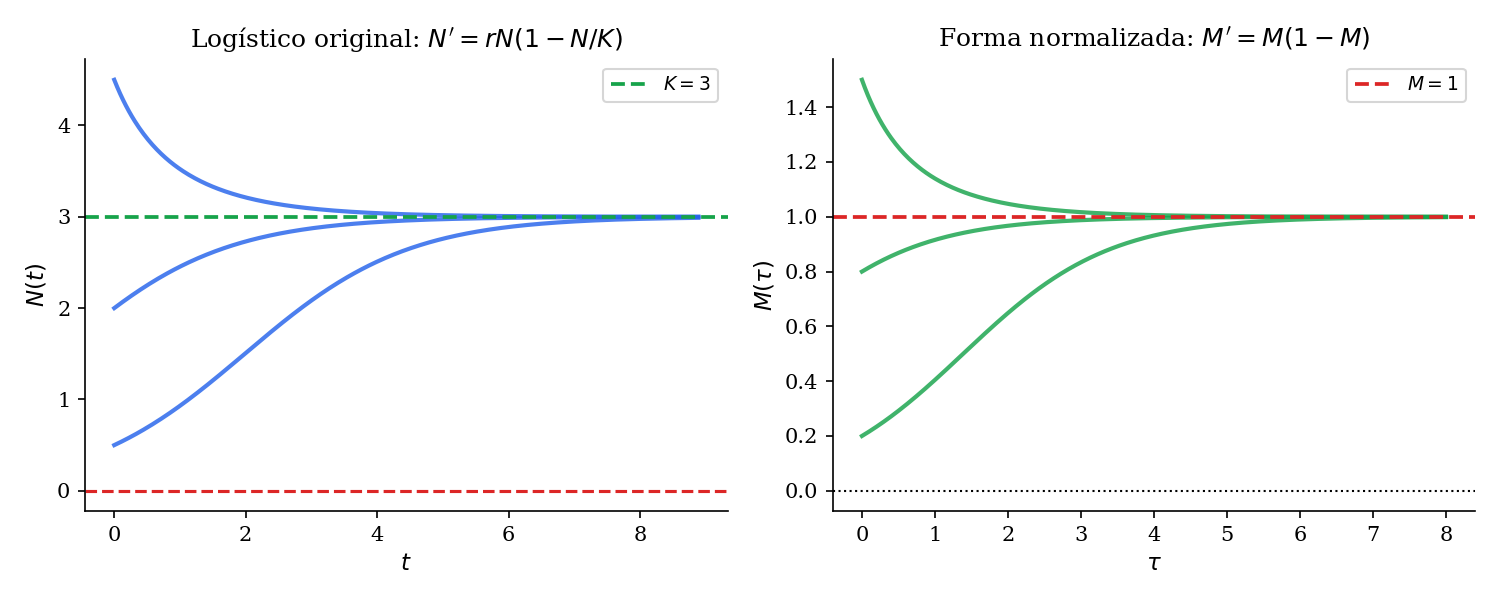
\includegraphics[width=0.88\textwidth]{fig_13_normalizacion_logistica.png}
\caption{Izquierda: logístico original $N'=rN(1-N/K)$.
Derecha: forma normalizada $\dot{u}=u(1-u)$ con $u=N/K$, $\tau=rt$.}
\end{figure}

\subsection{Análisis dimensional comparado}

\begin{center}
\begin{tabular}{lll}
\toprule
Ecuación & Variables con dimensión & Parámetros adimensionales\\
\midrule
$N'=rN(1-N/K)$ & $N$ ($\mathcal{N}$), $t$ ($T$) & $r$ ($T^{-1}$), $K$ ($\mathcal{N}$)\\
$\dot{u}=u(1-u)$ & --- & ninguno\\
$\dot{u}=u(1-u)-\lambda$ & --- & $\lambda=H/(rK)$\\
$\dot{u}=u(1-u)(u/\lambda-1)$ & --- & $\lambda=A/K$\\
\bottomrule
\end{tabular}
\end{center}

% ============================================================
\section{Dinámica de dos poblaciones: modelo general}
\label{sec:modelo-general-dos-poblaciones}
% ============================================================

La versión anterior de Lotka--Volterra se puede enriquecer incorporando
capacidad de carga en la presa y una respuesta funcional más general
$f(P)$:
\[
\frac{dP}{dt}=rP\!\left(1-\frac{P}{K}\right)-f(P)D,\qquad
\frac{dD}{dt}=-\gamma D+\delta f(P)D.
\]
El caso $f(P)=P$ recupera el sistema de Lotka--Volterra clásico, de modo que
esta formulación sirve como puente entre el modelo básico y sus variantes
ecológicas más realistas.

% ============================================================
\section{Problemas de la tarea (referencia)}
\label{sec:tarea-referencia}
% ============================================================

\subsection{EDOs: cinética química}

\begin{enumerate}
\item Sistema $A'=-kA$, $B'=kA$, $A(0)=A_0$, $B(0)=0$.
      Solución completa en la Sección~\ref{sec:cinetica} (reacción $A\to B$).
\item Sistema $A'=-2kA^2$, $B'=kA^2$, $A(0)=A_0$, $B(0)=0$.
      Solución completa en la Sección~\ref{sec:cinetica} (ley de acción de masas).
\end{enumerate}

\subsection{Estabilidad: modelo logístico}

Los incisos (a)--(e) quedan cubiertos en la Sección~\ref{sec:modelo-logistico}:
equilibrios, análisis geométrico, linealización, concordancia y solución analítica.

\subsection{Adimensionalización}

\begin{itemize}
    \item Problemas 1--3 (logístico, cosecha, Allee): Sección~\ref{sec:adimensionalizacion}.
    \item Problema 4 (caída libre con resistencia): Sección~\ref{sec:adimensionalizacion}.
    \item Problema 5 (oscilador amortiguado): Sección~\ref{sec:adimensionalizacion}.
    \item Problema 8 (Lotka--Volterra): Sección~\ref{sec:lotka-volterra}.
    \item Problema 10 (péndulo): Sección~\ref{sec:adimensionalizacion}.
    \item Problema 11 (circuito RC): Sección~\ref{sec:ecuaciones-lineales-primer-orden}.
\end{itemize}

\subsection{Bifurcaciones (al menos 5 de 10)}

La Sección~\ref{sec:bifurcaciones-unidim} cubre los tipos silla-nodo,
transcrítica, pitchfork supercrítica y pitchfork subcrítica con ejemplos
canónicos que corresponden directamente a los ejercicios (a), (b), (c), (d),
(f), (g), (h) de la tarea.

% ============================================================
\section{Notas de legibilidad del material original}
% ============================================================

\begin{itemize}
    \item Algunas etiquetas de unidades en las esquinas de las primeras páginas
          del material manuscrito no son completamente legibles.
    \item Algunas frases auxiliares de los diagramas de campo de pendientes no
          se distinguen con suficiente precisión.
    \item Las páginas 4, 5 y 10 del PDF revisado aparecen prácticamente vacías
          o negras; su contenido se infirió del contexto matemático.
\end{itemize}

\end{document}
